\documentclass[../main-report.tex]{subfiles}
\begin{document}
\section{Một số lý thuyết về xác suất}
% Tham khảo: https://machinelearningcoban.com/2017/07/09/prob/
Có thể nói một điều rằng lý thuyết xác suất là một trong những lý thuyết quan trọng nhất của khoa học hiện đại và đặc biệt là \textbf{Machine Learning} bởi vì đa phần các thuật toán của Machine Learning đều có cơ sở dựa trên xác suất.

Phần bên dưới chúng tôi trình bày chủ yếu một số lý thuyết cơ bản được chúng tôi tìm hiểu và tổng hợp từ \citep{MLCB:xacsuat}
\subsection{Không gian xác suất}
Khi nói đến xác suất là người ta nói đến các lý thuyết toán học về sự \textit{bất định - uncertainly} hay nói một cách khác, xác suất biểu thị khả năng xảy ra của các \textit{sự kiện - event} trong một môi trường bất định nào đó. Ví dụ chúng ta xét về xác suất có mưa hay không có mưa vào thứ hai tuần tới, xác suất tỏ tình thành công hay thất bại của cậu bạn thân,\ldots Tóm lại cứ nói đến xác suất là đề cập đến sự không chắc chắn hay bất định đó.

Về mặt toán học, người ta kí hiệu một \textbf{không gian xác suất - probability space} bao gồm 3 thành phần $(\Omega, F, P)$ như sau:

\begin{itemize}
\item $\Omega$ (có thể đọc là ``Ô-me-ga'') chính là tập các giá trị \textbf{có thể xảy ra - possible outcome} với sự kiện trong không gian xác suất. Người ta còn gọi nó là \textbf{không gian mẫu}.
\item $F \subseteq 2^{\Omega}$ là tập hợp các sự kiện có thể xảy ra trong không gian xác suất.
\item $P$ là xác suất (hoặc phân phối xác suất) của sự kiện. $P$ ánh xạ một sự kiện $E \in F$ vào trong một giá trị thực $p \in \left [ 0;1 \right ]$. Ở đây chúng ta gọi $p = P(E)$ là xác suất của sự kiện $E$.
\end{itemize}

\subsubsection*{Ví dụ minh họa}
Chúng ta cùng nhau xem xét một ví dụ khá kinh điển trong lý thuyết xác suất đó chính là ví dụ \textbf{tung xúc sắc}.

Giả sử rằng chúng ta tung một con xúc sắc 6 mặt. Không gian các \textbf{outcomes} có thể xảy ra trong trường hợp này là $\Omega = \left \{ 1, 2, 3, 4, 5, 6 \right \}$ - chúng ta không tính đến các trường hợp xúc sắc rơi lơ lửng tức là không thuộc mặt nào. Không gian các sự kiện $F$ sẽ tùy thuộc vào sự định nghĩa của chúng ta. Ví dụ chúng ta định nghĩa sự kiện xúc sắc là mặt chẵn hoặc mặt lẻ thì không gian sự kiện $F=\left \{ \varnothing , \left \{ 1, 3, 5 \right \}, \left \{ 2, 4, 6 \right \}, \Omega \right \}$ trong đó $\varnothing$ là sự kiện có xác suất 0 - hay còn gọi là biến cố \textit{không thể có}. $\Omega$ là sự kiện có xác suất 1 - hay còn gọi là \textit{biến cố chắc chắn}.
\subsection{Các tính chất xác suất}
Giống như ví dụ ở phía trên, khi \textit{không gian mẫu - outcomes space} là hữu hạn thì chúng ta thường lựa chọn không gian sự kiện $F=2^{\Omega} = \left \{ \varnothing , \left \{ 1, 3, 5 \right \}, \left \{ 2, 4, 6 \right \}, \Omega \right \}$. Cách tiếp cận này chưa hẳn đã tổng quát hóa cho mọi trường hợp tuy nhiên nó đủ dùng trong các bài toán thực tế, tất nhiên là với giả thiết không gian mẫu của chúng ta là \textbf{hữu hạn}. Khi không gian mẫu là\textbf{ vô hạn - infinite} chúng ta phải hết sức cẩn thận trong việc lựa chọn không gian sự kiện $F$. Khi đã định nghĩa được không gian sự kiện $F$ thì hàm xác suất của chúng ta bắt buộc phải thỏa mãn các tính chất sau đây:

\begin{itemize}
\item \textbf{Không âm - non-negativity} - xác suất của mọi sự kiện là không âm, tức là với mọi $x \in F,~~ P(x)\geq 0$
\item \textbf{Xác suất toàn cục - trivial event} $P(\Omega) = 1$
\item \textbf{Tính cộng - additivity} tức là với mọi $x, y \in F$ nếu như $x\cap y= \varnothing$ thì ta có $P(x\cup y) = P(x) + P(y)$
\end{itemize}

\subsection{Biến ngẫu nghiên}
\textbf{Biến ngẫu nghiên (Random Variables)} là một thành phần quan trọng trong lý thuyết xác suất. Nó biểu diễn giá trị của các đại lượng không xác định, thông thường nó được coi như một ánh xạ từ tập các \textbf{outcomes} trong không gian mẫu thành các giá trị thực.

\begin{figure}[ht!]
\centering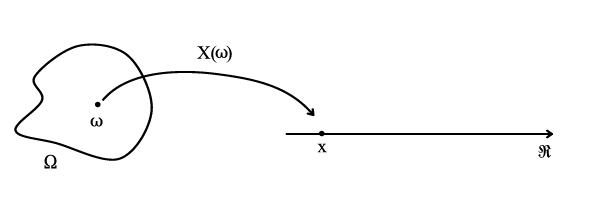
\includegraphics[scale=0.9]{random-variable}
\caption{Minh họa giá trị X ánh xạ từ các tập outcomes}
\end{figure}

Quay trở lại với ví dụ tung xúc sắc phía trên, gọi $X$ là biến ngẫu nhiên biểu diễn kết quả của các những lần gieo xúc sắc. Một lựa chọn khá tự nhiên và đơn giản đó là: \textbf{``$\boldsymbol{X}$ là số chấm tròn trên mặt tung được''}

Chúng ta cũng có thể lựa chọn một chiến lược biểu diễn biến ngẫu nhiên $X$ khác chẳng hạn như sau:

\begin{equation} \label{eq:ex_rand_var}
X = \left\{\begin{array}{ll}
	1 & \text{ if i is odd} \\
	0 & \text{ if i is even}
	\end{array}\right.
\end{equation}

Có nghĩa là cùng một biến cố nhưng biểu diễn nó như thế nào là việc của mỗi chúng ta. Biến ngẫu nhiên $X$ biểu diễn như biểu thức (\ref{eq:ex_rand_var}) được gọi là \textit{binary random variables - biến nhị phân}. Biến nhị phân được sử dụng rất thông dụng trong thực tế công việc nhất là Machine Learning và thường được biết đến với cái tên \textbf{indicator variables} nó thể hiện s\textit{ự xảy ra hay không xảy ra} của một sự kiện.

\subsubsection*{Biến ngẫu nhiên rời rạc và biến ngẫu nhiên liên tục}
Có hai loại biến ngẫu nhiên đó là \textbf{BNN rời rạc} (discrete) và \textbf{BNN liên tục} (continuous).

\textbf{Rời rạc} có thể hiểu một cách đơn giản là giá trị của nó thuộc vào một tập định trước. 
Ví dụ tung đồng xu thì có hai khả năng là head và tail \footnote{Tên gọi này bắt nguồn từ đồng xu Mỹ, một mặt có hình mặt người, được gọi là \textit{head}, trái ngược với mặt này được gọi là mặt \textit{tail}, cách gọi này hay hơn cách gọi \textit{xấp ngử}a vì ta không có quy định rõ ràng thế nào là xấp ngay ngửa}. Tập các giá trị này có thể là có thứ tự (khi tung xúc xắc) hoặc không có thứ tự (unorderd), ví dụ khi đầu ra là các giá trị \textit{nắng, mưa, bão},\ldots. Mỗi đầu ra có một giá trị xác suất tương ứng với nó. Trong Machine Learning các giá trị này tương ứng với \textit{các phân lớp (class)}. Các giá trị xác suất này không âm và có tổng bằng một:

\begin{equation}
\sum_{\forall x}{p(x)}=1 
\end{equation}

Còn \textbf{biến ngẫu nhiên liên tục} có thể định nghĩa là các biến ngẫu nhiên mà các giá trị của nó rơi vào một tập \textit{không biết trước}. Trong Machine Learning người ta gọi lớp bài toán với biến ngẫu nhiên liên tục là \textbf{Hồi quy}. Giá trị của nó có thể nằm trong một khoảng hữu hạn ví dụ như thời gian làm bài thi đại học là $t \in \left ( 0;180 \right )$ phút hoặc cũng có thể là vô hạn ví dụ như thời gian từ bây giờ đến ngày tận thế $t \in \left ( 0; +\infty \right )$ chẳng hạn. Khi đó hàm mật độ xác suất của nó trên toàn miền giá trị $D$ của outcomes space được định nghĩa bằng một tích phân như sau:

\begin{equation}
\int_{D}p(x)dx=1
\end{equation}

\subsection{Xác suất có điều kiện}
Dựa vào phổ điểm của các học sinh, liệu ta có thể tính được xác suất để một học sinh được điểm 10 môn Lý, biết rằng học sinh đó được điểm 1 môn Toán (ai cũng có quyền hy vọng). Hoặc biết rằng bây giờ đang là tháng 7, tính xác suất để nhiệt độ hôm nay cao hơn 30 độ C.

Xác suất có điều kiện (\textbf{conditional probability}) của một biến ngẫu nhiên $x$ biết rằng biến ngẫu nhiên $y$ có giá trị $y^{*}$ được ký hiệu là $p(x | y = y^{*})$ (đọc là ``\textit{xác suất của} $x$ \textit{biết} $y$ \textit{có giá trị} $y^{*}$'' - \textit{probability of} $x$ \textit{given that} $y$ \textit{takes value} $y^{*}$ ).

Xác suất có điều kiện \(p(x | y = y^*)\) có thể được tính dựa trên \textit{joint probobability} \(p(x, y)\) \footnote{Xác suất hợp (\textit{Joint probability}) là xác suất của hai biến cố cùng xảy ra.}. Tổng quát ta có công thức để tính như sau:

\begin{equation}
  p(x | y = y^*) = \frac{p(x, y = y^*)}{\sum_{x} p(x, y = y^*)} = \frac{p(x, y = y^*)}{p(y = y^*)}
\end{equation}

Thông thường, ta có thể viết xác suất có điều kiện mà không cần chỉ rõ giá trị \(y = y^*\) và có công thức gọn hơn:

\begin{equation}
	p(x | y) = \frac{p(x, y)}{p(y)}
\end{equation}
  
Tương tự:

\begin{equation}
  p(y | x) = \frac{p(y, x)}{p(x)}
\end{equation}

Và ta sẽ có quan hệ:

\begin{equation} \label{eq:join_prob}
  p(x, y) = p(x | y)p(y) = p(y | x)p(x)
\end{equation}

Khi có nhiều hơn hai biến ngẫu nhiên, ta có các công thức:


\begin{eqnarray}
  p(x, y, z, w)
  & = & p(x, y, z | w) p(w) \\
  & = & p(x, y | z, w)p(z, w) = p(x, y | z, w) p(z | w) p(w) \quad \\
  & = & p(x | y, z, w)p(y | z, w)p(z | w) p(w) \label{eq:conditional_prob}
\end{eqnarray}

Công thức \(\ref{eq:conditional_prob}\) có dạng chuỗi (\textit{chain}) và được sử dụng nhiều sau này.

\subsection{Quy tắc Bayes}
Công thức (\ref{eq:join_prob}) biểu diễn \textit{joint probability} theo hai cách. Từ đây ta có thể suy ra quan hệ giữa hai \textit{conditional probabilities} \(p(x |y)\) và \(p(y | x)\):

\[
  p(y | x) p(x) = p(x | y) p(y)
\]

Biến đối một chút:


\begin{eqnarray}
  p(y | x)
  & = & \frac{p(x | y) p(y)}{p(x)} \label{eq:bayes_1} \\
  & = & \frac{p(x | y) p(y)}{\sum_{y} p(x, y)} \\
  & = & \frac{p(x |y) p(y)}{\sum_{y} p(x | y) p(y)} \quad \label{eq:bayes_2}
\end{eqnarray}

Từ (\ref{eq:bayes_2}) ta có thể thấy rằng \(p(y | x)\) hoàn toàn có thể tính được nếu ta biết mọi \(p(x | y)\) và \(p(y)\). Tuy nhiên, việc tính trực tiếp xác suất này thường là phức tạp. Thay vào đó, ta có thể đi tìm mô hình phù hợp của \(p(\mathbf{x} | y)\) trên training data sao cho \textit{những gì đã thực sự xảy ra có xác suất cao nhất có thể}. Dựa trên training data, các tham số của mô hình này có thể tìm được qua một \textit{bài toán tối ưu}.

\textbf{Ba công thức (\ref{eq:bayes_1}) - (\ref{eq:bayes_2}) thường được gọi là Quy tắc Bayes (Bayes' rule). Quy tắc này rất quan trọng trong Machine Learning!}

Trong Machine Learning, chúng ta thường mô tả quan hệ giữa hai biến \(x\) và \(y\) dưới dạng xác suất có điều kiện \(p(x|y)\). Ví dụ, biết rằng đầu vào là một bức ảnh ở dạng vector \(\vec{x}\), xác suất để bức ảnh chứa một chiếc xe là bao nhiêu. Khi đó, ta phải tính \(p(y | \vec{x})\).

\subsubsection*{Độc lập (Independence)}
Nếu biết giá trị của một biến ngẫu nhiên \(x\) không mang lại thông tin về việc suy ra giá trị của biến ngẫu nhiên \(y\) (và ngược lại), thì ta nói rằng hai biến ngẫu nhiên là \emph{độc lập} (independence). Chẳng hạn, chiều cao của một học sinh và điểm thi môn Toán của học sinh đó có thể coi là hai biến ngẫu nhiên độc lập.

Khi hai biến ngẫu nhiên \(x\) và \(y\) là \emph{độc lập}, ta sẽ có:


\begin{eqnarray}
  p(x | y) &=& p(x) \quad \\
  p(y | x) &=& p(y)
\end{eqnarray}


Thay vào biểu thức Conditional Probability trong (\ref{eq:join_prob}), ta có:

\begin{equation}
	p(x, y) = p(x | y) p(y) = p(x) p(y)
\end{equation}


\subsection{Kỳ vọng}
\textbf{Kỳ vọng (expectation)} của một biến ngẫu nhiên được định nghĩa là:


\begin{eqnarray}
  \text{E}[x] = \sum_x x p(x) \quad & \text{if}~ x ~ \text{is discrete} \quad \\
  \text{E}[x] = \int x p(x) dx \quad & \text{if}~ x ~ \text{is continuous}
\end{eqnarray}

Giả sử \(f\) là một hàm số trả về một giá trị với mỗi giá trị \(x^*\) của biến ngẫu nhiên \(x\). Khi đó, nếu \(x\) là biến ngẫu nhiên rời rạc, ta sẽ có:

\begin{equation}
	\text{E}[f(x)] = \sum_x f(x) p(x)
\end{equation}

Công thức cho biến ngẫu nhiên liên tục cũng được viết tương tự.

Với joint probability:

\begin{equation}
\text{E}[f(x, y)] = \sum_{x,y} f(x, y) p(x, y) dx dy
\end{equation}

Có 3 quy tắc cần nhớ về kỳ vọng:

\begin{enumerate}
\item Kỳ vọng của một hằng số theo một biến ngẫu nhiên \(x\) bất kỳ bằng chính hằng số đó:

\begin{equation}
\text{E}[\alpha] = \alpha
\end{equation}

\item Kỳ vọng có tính chất tuyến tính:

\begin{eqnarray}
  \text{E}[\alpha x] & = & \alpha \text{E}[x] \quad \\
  \text{E}[f(x) + g(x)] & = & \text{E}[f(x)] + \text{E}[g(x)]
\end{eqnarray}

\item Kỳ vọng của tích hai biến ngẫu nhiên bằng tích kỳ vọng của hai biến đó \textbf{nếu hai biến ngẫu nhiên đó là độc lập}. Điều ngược lại không đúng:

\begin{equation}
\text{E}[f(x) g(y)] = \text{E}[f(x)] \text{E}[g(y)]
\end{equation}

\end{enumerate}
\subsection{Một vài phân phối xác suất thường gặp}
\subsubsection*{Phân phối Bernouli}
\textbf{Phân phối Bernoulli (Bernouli distribution)} là một phân bố rời rạc mô tả biến ngẫu nhiên nhị phân: nó mô tả trường hợp khi đầu ra chỉ nhận một trong hai giá trị \(x \in \{0, 1\}\). Hai giá trị này có thể là \emph{head} và \emph{tail} khi tung đồng xu; có thể là \emph{fraud transaction} và \emph{normal transaction} trong bài toán xác định giao dịch lừa đảo trong tín dụng; có thể là \emph{người} và \emph{không phải người} trong bài toán tìm xem trong một bức ảnh có người hay không.

Bernoulli distribution được mô tả bằng một tham số \(\lambda \in [0, 1]\) và là xác suất để \(x = 1\). Phân bố của mỗi đầu ra sẽ là:

\begin{equation}
p(x = 1) = \lambda, ~~~~ p(x = 0) = 1 - p(x = 1) = 1 - \lambda
\end{equation}

Hai đẳng thức này thường được viết gọn lại:

\begin{equation}
p(x) = \lambda^x (1 - \lambda)^{1 - x}
\end{equation}

với giả định rằng \(0 ^0 = 1\).

Bernoulli distribution được ký hiệu ngắn gọn dưới dạng:
\[
  p(x) = \text{Bern}_x [\lambda]
\]

\subsubsection*{Phân phối tổng quát của Bernouli (Categorical distribution)}
Cũng là biến ngẫu nhiên rời rạc, nhưng trong hầu hết các trường hợp, đầu ra có thể là một trong nhiều hơn hai giá trị khác nhau. Ví dụ, một bức ảnh có thể chứa một chiếc xe, một người, hoặc một con mèo. Khi đó, ta dùng phân bố tổng quát của Bernoulli distribution và được gọi là \emph{Categorical distribution}. Các đầu ra được mô tả bởi 1 phần tử trong tập \(\{1, 2, \dots, K\}\).

Nếu có \(K\) đầu ra có thể đạt được, Categorical distribution sẽ được mô tả bởi \(K\) tham số, viết dưới dạng vector: \(\lambda = [\lambda_1, \lambda_2, \dots, \lambda_K]\) với các \(\lambda_k\) không âm và có tổng bằng 1. Mỗi giá trị \(\lambda_k\) thể hiện xác suất để đầu ra nhận giá trị \(k\):

\[
  p(x = k) = \lambda_k
\]

Viết gọn lại:

\[
  p(x) = \text{Cat}_x [\lambda]
\]

Biểu diễn theo cách khác, ta có thể coi như đầu ra là một vector ở dạng \emph{one-hot} vector, tức \(\mathbf{x} \in \{\mathbf{e}_1, \mathbf{e}_2, \dots, \mathbf{e}_K\}\) với \(\mathbf{e}_k\) là vector đơn vị thứ \(k\), tức tất cả các phần tử bằng 0, trừ phần tử thứ \(k\) bằng 1. Khi đó, ta sẽ có:

\begin{equation}
p(\mathbf{x} = \mathbf{e}_k) = \prod_{j=1}^K \lambda_j^{x_j} = \lambda_k
\end{equation}

Cách viết này được sử dụng rất nhiều trong Machine Learning.

\subsubsection*{Phân phối chuẩn một biến (Univariate normal distribution)}
\textbf{Phân phối chuẩn 1 biến (univariate normal hoặc Gaussian distribution)} được định nghĩa trên các biến liên tục nhận giá trị \(x \in (-\infty, \infty)\).

Phân phối này được mô tả bởi hai tham số: \emph{mean} \(\mu\) và \emph{variance} \(\sigma^2\). Giá trị \(\mu\) có thể là bất kỳ số thực nào, thể hiện vị trí của \emph{peak}, tức tại đó mà hàm mật độ xác suất đạt giá trị cao nhất. Giá trị \(\sigma^2\) là một giá trị dương, với \(\sigma\) thể hiện \emph{độ rộng} của phân bố này. \(\sigma\) lớn chứng tỏ khoảng giá trị đầu ra biến đổi mạnh, và ngược lại.

Hàm mật độ xác suất của phân phối này được định nghĩa là:

\begin{equation}
  p(x) = \frac{1}{\sqrt{2\pi \sigma^2}}\exp \left( -\frac{(x - \mu)^2}{2\sigma^2}\right)
\end{equation}

Dạng gọn hơn:

\begin{equation}
p(x) = \text{Norm}_x [\mu, \sigma^2]
\end{equation}

\section{Giới thiệu Machine Learning}
\subsection{Khái niệm}
Trên Wikipedia tiếng Anh họ có định nghĩa về machine learning như sau:

\begin{quote}
``\textbf{Machine learning} is a subset of artificial intelligence in the field of computer science that often uses statistical techniques to give computers the ability to `learn' (i.e., progressively improve performance on a specific task) with data, without being explicitly programmed'' \citep{wiki:machine_learning}
\end{quote}

Chúng ta có thể hiểu đơn giản định nghĩa ở trên như sau: 

\textbf{Machine learning} là một lĩnh vực nhỏ của trí tuệ nhân tạo (\textit{Artificial Intelligence - AI}) trong khoa học máy tính, nó thường sử dụng các kĩ thuật thống kê để máy tính có khả năng `học' với dữ liệu, mà không cần phải lập trình cụ thể.

\subsection{Phân loại}

\section{Thuật toán Decision Tree}
\subsection{Giới thiệu}
Sắp đến kỳ thi, một cậu sinh viên tự đặt ra quy tắc \textit{học hay chơi} của mình như sau:

\begin{itemize}
\item Nếu còn nhiều hơn hai ngày tới ngày thi, cậu sẽ đi chơi.
\item Nếu còn không quá hai ngày và đêm hôm đó có một trận bóng đá, cậu sẽ sang nhà bạn chơi và cùng xem bóng đêm đó.
\item Cậu sẽ chỉ học trong các trường hợp còn lại.
\end{itemize}

Việc ra quyết định của cậu sinh viên này có thể được mô tả trên sơ đồ trong hình \ref{fig:dt_ex1}.

\begin{figure}[ht!]
\centering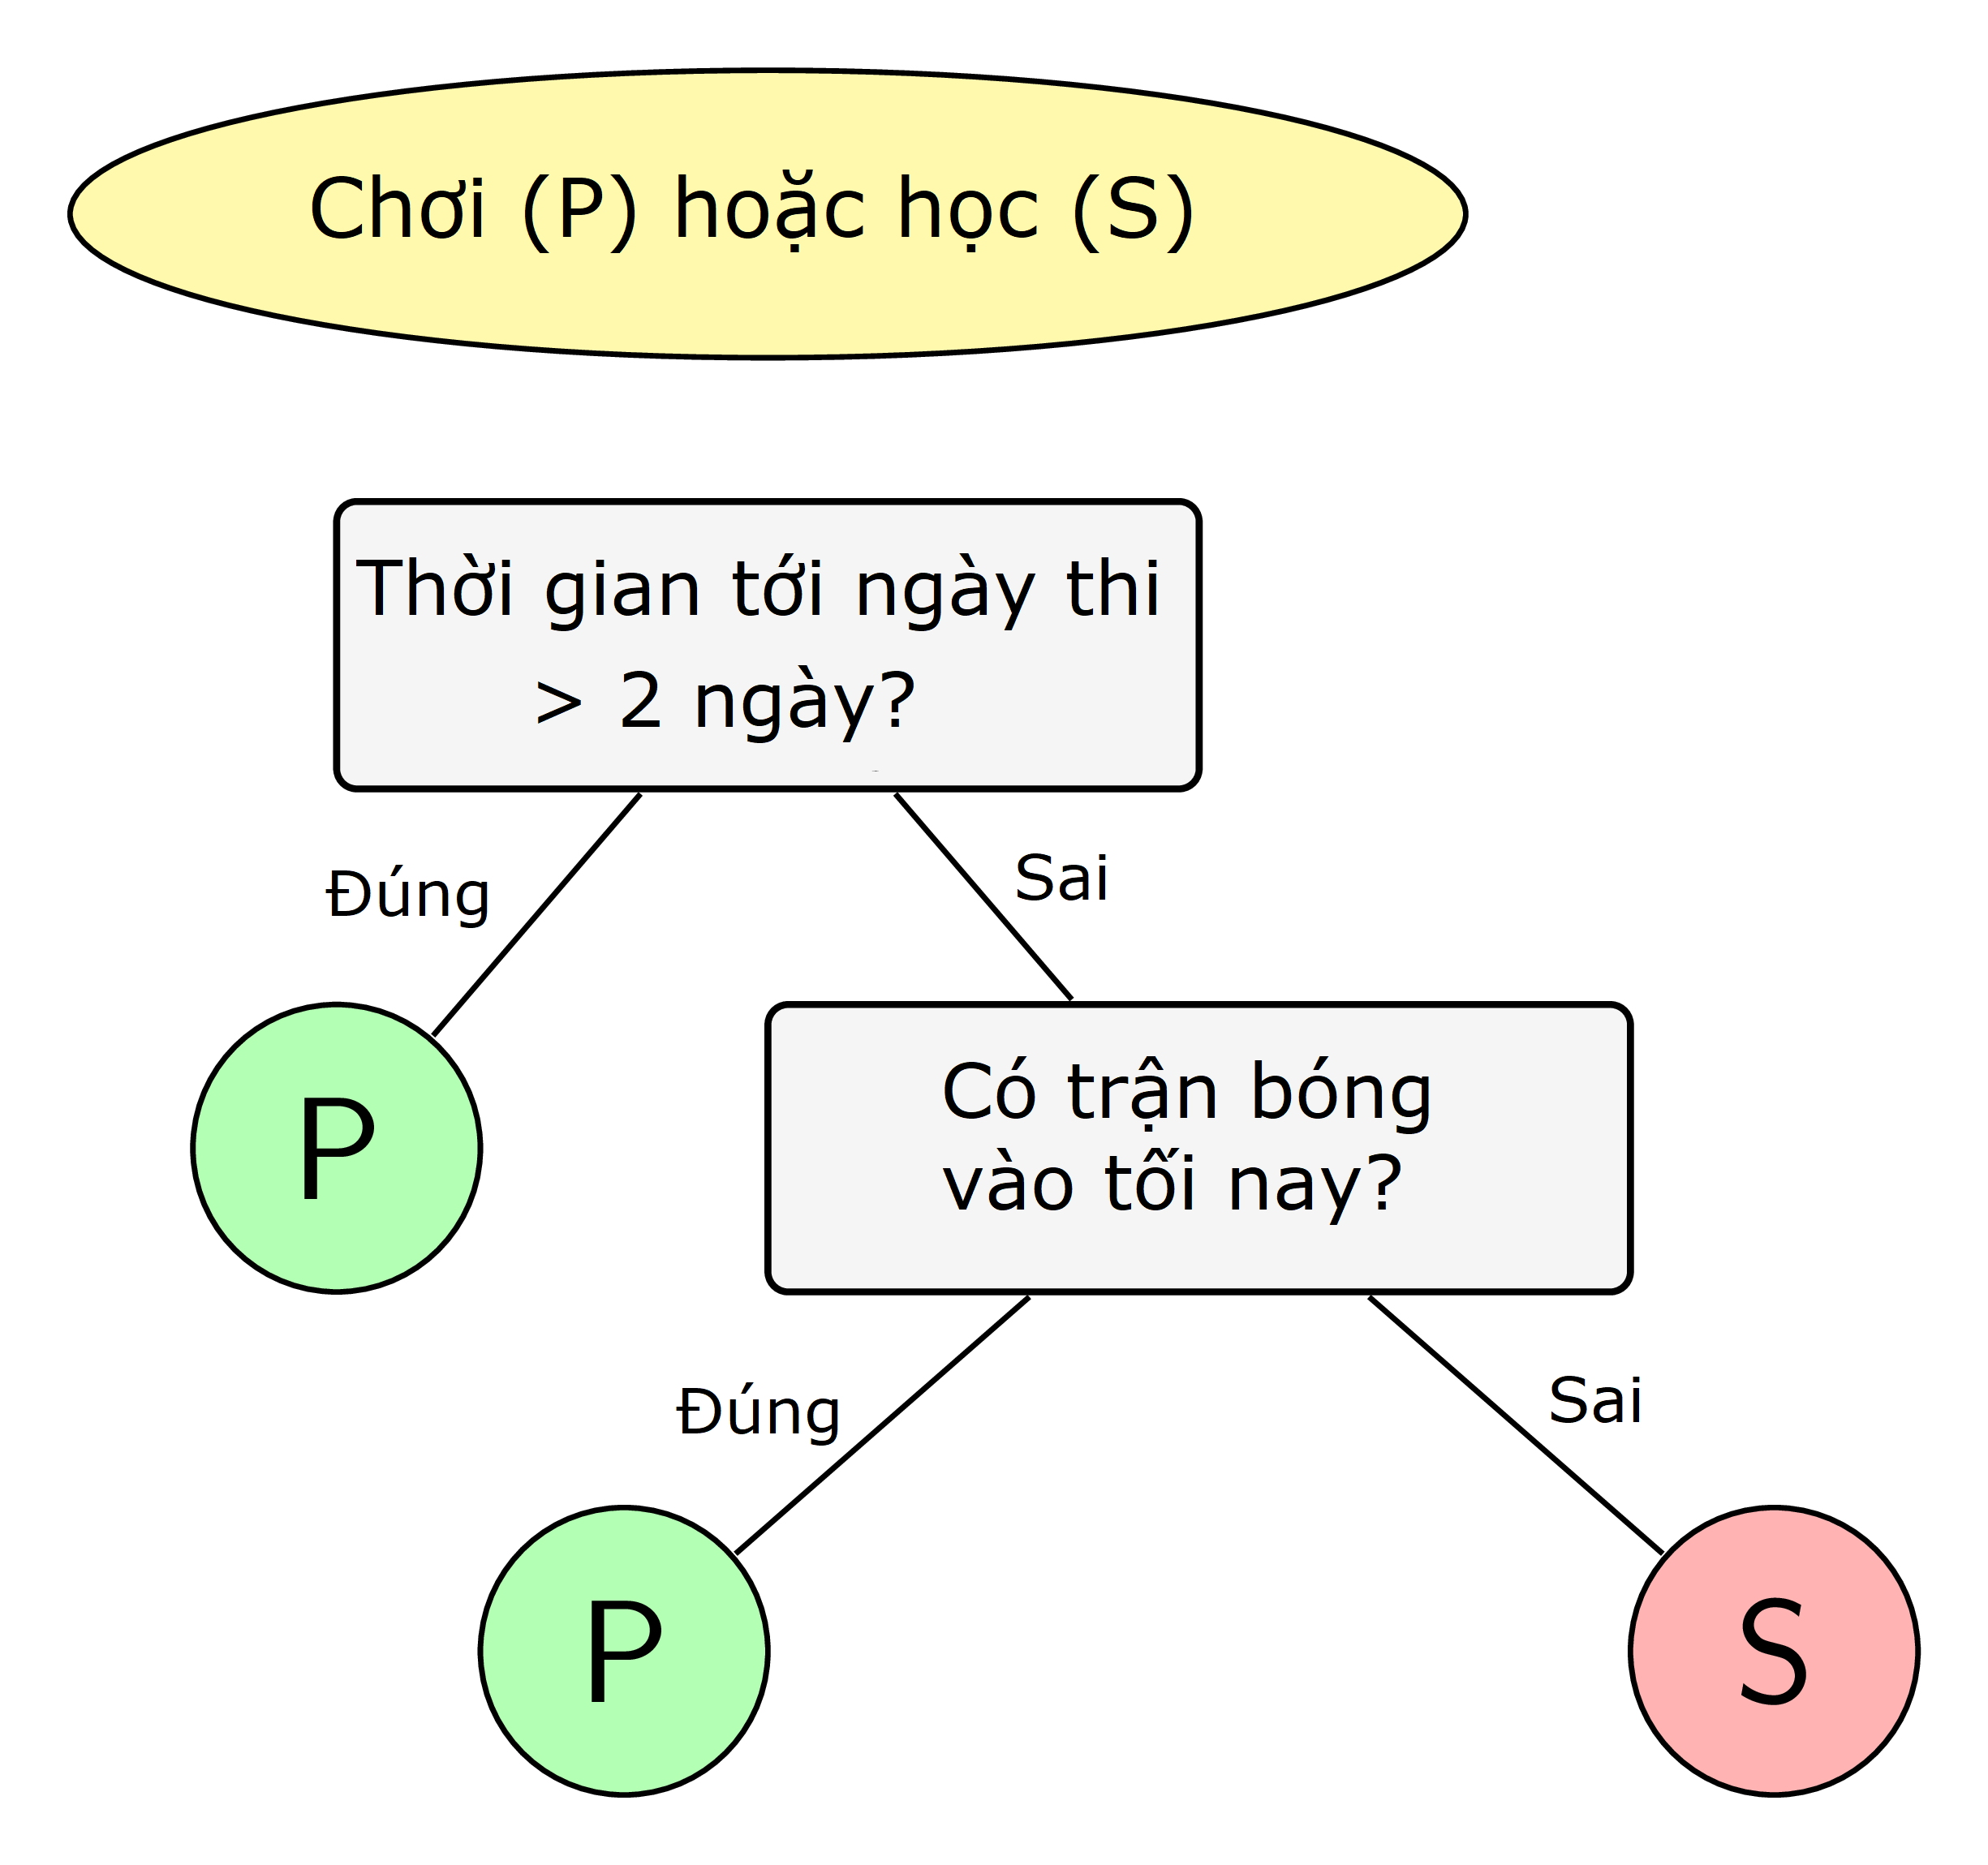
\includegraphics[scale=0.1]{dt_ex1}
\caption{Một ví dụ về việc đưa ra các quyết định dựa trên câu hỏi}
\label{fig:dt_ex1}
\end{figure}

Hình ellipse nền vàng thể hiện quyết định cần được đưa ra. Quyết định này phụ thuộc vào các câu trả lời của các câu hỏi trong các ô hình chữ nhật màu xám. Dựa trên các câu trả lời, quyết định cuối cùng được cho trong các hình tròn màu lục (chơi) và đỏ (học).

Việc quan sát, suy nghĩ và ra các quyết định của con người thường được bắt đầu từ các câu hỏi. Machine learning cũng có một mô hình ra quyết định dựa trên các câu hỏi. Mô hình này có tên là \textit{cây quyết định (decision tree)}.

Trong \textbf{decision tree}, các ô màu xám, lục, đỏ trên hình \ref{fig:dt_ex1} được gọi là các node. Các node thể hiện đầu ra (màu lục và đỏ) được gọi là \textit{node lá} (\textit{leaf node} hoặc \textit{terminal node}). Các node thể hiện câu hỏi là các \textit{non-leaf node}. Non-leaf node trên cùng (câu hỏi đầu tiên) được gọi là node gốc (\textit{root node}). Các non-leaf node thường có hai hoặc nhiều node con (\textit{child node}). Các child node này có thể là một leaf node hoặc một non-leaf node khác. Các child node có cùng bố mẹ được gọi là \textit{sibling node}. Nếu tất cả các non-leaf node chỉ có hai child node, ta nói rằng đó là một \textit{binary decision tree} (cây quyết định nhị phân). Các câu hỏi trong binary decision tree đều có thể đưa được về dạng câu hỏi đúng hay sai. Các decision tree mà một leaf node có nhiều child node cũng có thể được đưa về dạng một binary decision tree. Điều này có thể đạt được vì hầu hết các câu hỏi đều có thể được đưa về dạng câu hỏi đúng sai.

Ví dụ, ta có thể xác định được tuổi của một người dựa trên nhiều câu hỏi đúng sai dạng: tuổi của bạn lớn hơn $x$ đúng không? (Đây chính là thuật toán \textit{tìm kiếm nhị phân – binary search}.)

Decision tree là một mô hình \textit{supervised learning}, có thể được áp dụng vào cả hai bài toán \textit{classification và regression}. Việc xây dựng một decision tree trên dữ liệu huấn luyện cho trước là việc đi xác định các câu hỏi và thứ tự của chúng. Một điểm đáng lưu ý của decision tree là nó có thể làm việc với các đặc trưng (trong các tài liệu về decision tree, các đặc trưng thường được gọi là thuộc tính – \textit{attribute}) dạng \textit{categorical}, thường là rời rạc và không có thứ tự. Ví dụ, mưa, nắng hay xanh, đỏ, v.v. Decision tree cũng làm việc với dữ liệu có vector đặc trưng bao gồm cả thuộc tính dạng categorical và liên tục (numeric). Một điểm đáng lưu ý nữa là decision tree ít yêu cầu việc chuẩn hoá dữ liệu.

\subsection{Phân loại}
Có 3 loại decision trees phổ biến sau:

\begin{itemize}
\item \textbf{ID3 (Iterative Dichotomiser 3)} - Tạo cây nhiều chiều, tìm cho mỗi node một đặt tính phân loại sao cho đặt tính này có giá trị ``information gain'' lớn nhất. Cây được phát triển tới mức tối đa kích thước. Sau đó áp dụng phương thức cắt tỉa cành để xử lý những dữ liệu chưa nhìn thấy.
\item \textbf{C4.5} - Kế thừa từ  ID3 nhưng loại bỏ hạn chế về việc chỉ sử dụng đặc tính có giá trị phân loại bằng cách tự động định nghĩa một thuộc tính rời rạc. Dùng để phân chia những thuộc tính liên tục thành những tập rời rạc.
\item \textbf{CART (Classification and Regression Trees)} - Tương tự như C4.5, nhưng nó hỗ trợ thêm đối tượng dự đoán là giá trị số (\textit{Regression}). Cấu trúc CART dạng cây nhị phân, mỗi node sử dụng một ngưỡng để đạt được ``information gian'' lớn nhất.
\end{itemize}

Hình \ref{fig:decision_tree_type_comparison} so sánh giữa các loại thuật toán decision tree.

\begin{figure}[ht!]
\centering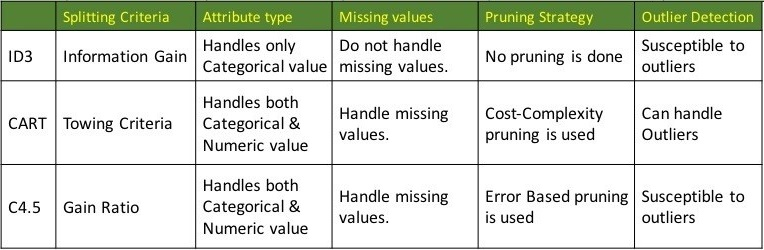
\includegraphics[scale=0.75]{comparison-decision-trees}
\caption{So sánh các thuật toán Decision Trees}
\label{fig:decision_tree_type_comparison}
\end{figure}

\subsection{Ưu và nhược điểm của thuật toán}
Tùy vào loại Decision tree sử dụng mà ta có ưu nhược điểm riêng. Nhưng nhìn chung thuật toán có những ưu nhược điểm chung như sau:
\subsubsection*{Về ưu điểm}
\begin{itemize}
\item Decision tree thường mô phỏng cách suy nghĩ con người. Vì vậy nó đơn giản để hiểu và diễn giải dữ liệu.
\item Giúp ta nhìn thấy được sự logic của dữ liệu ( không như thuật toán phần laoij SVM, KNN …)
\item Có khả năng chọn được những features tốt nhất.
\item Phân loại dữ liệu không cần tính toán phức tạp.
\item Giải quyết vấn đề nhiễu và thiếu dữ liệu.
\item Có khả năng xử lý dữ liệu có biến liên tục và rời rạc.
\end{itemize}

\subsubsection*{Về nhược điểm}
\begin{itemize}
\item Tỉ lệ tính toán tăng theo hàm số mũ còn vấn đề ngày càng lớn hơn.
\item Dễ bị vấn đề overfitting và high bias khi tập dữ liệu huấn luyện nhỏ.
\end{itemize}

Trong bài báo cáo này chúng tôi sử dụng loại \textbf{CART}. Do tính đơn giản, dể tiếp cận của nó, cũng như những giá trị feature mà ta sử dụng là kiểu dữ liệu biến liên tục không phải phân loại nên không dùng \textbf{ID3} được. Và đây là loại decision tree được thư viện \textit{scikit-learn} chọn sử dụng.
\subsection{Làm sạch dữ liệu}

\subsection{Quá trình xây dựng cây}

\section[Một số lỗ hổng web]{Một số lỗ hổng tấn công web phổ biến}
\subsection{SQL Injection}

\subsection{Cross-Site Scripting (XSS)}

\end{document}